\documentclass[11pt, A4paper,norsk]{article}
\usepackage[utf8]{inputenc}
\usepackage[T1]{fontenc}
\usepackage{babel}
\usepackage{amsmath}
\usepackage{amsfonts}
\usepackage{amsthm}
\usepackage[colorlinks]{hyperref}
\usepackage{listings}
\usepackage{color}
\usepackage{hyperref}
\usepackage{graphicx}
\usepackage{cite}
\usepackage{float}

\definecolor{dkgreen}{rgb}{0,0.6,0}
\definecolor{gray}{rgb}{0.5,0.5,0.5}
\definecolor{daynineyellow}{rgb}{1.0,0.655,0.102}
\definecolor{url}{rgb}{0.1,0.1,0.4}

\lstset{frame=tb,
	language=Python,
	aboveskip=3mm,
	belowskip=3mm,
	showstringspaces=false,
	columns=flexible,
	basicstyle={\small\ttfamily},
	numbers=none,
	numberstyle=\tiny\color{gray},
	keywordstyle=\color{blue},
	commentstyle=\color{daynineyellow},
	stringstyle=\color{dkgreen},
	breaklines=true,
	breakatwhitespace=true,
	tabsize=3
}

\lstset{inputpath="C:/Users/Torstein/Documents/UiO/Fys-mek1110/Python programmer/Oblig3"}
\graphicspath{{C:/Users/Torstein/Documents/UiO/Fys-mek1110/"Python programmer"/Oblig3/}}
\hypersetup{colorlinks, urlcolor=url}

\author{Torstein Solheim Ølberg}
\title{Svar på Oblig nr. 3 i Fys-Mek1110}

\begin{document}
\maketitle
	\begin{center}
\Large \textbf{Oppgaver}
	\end{center}









		\paragraph{a)}
			\begin{flushleft}
Draw a free-body diagram for the block. \\
\vspace{1mm}
\textbf{Løsning:}
\vspace{1mm}
			\end{flushleft}
			\begin{figure}[H]
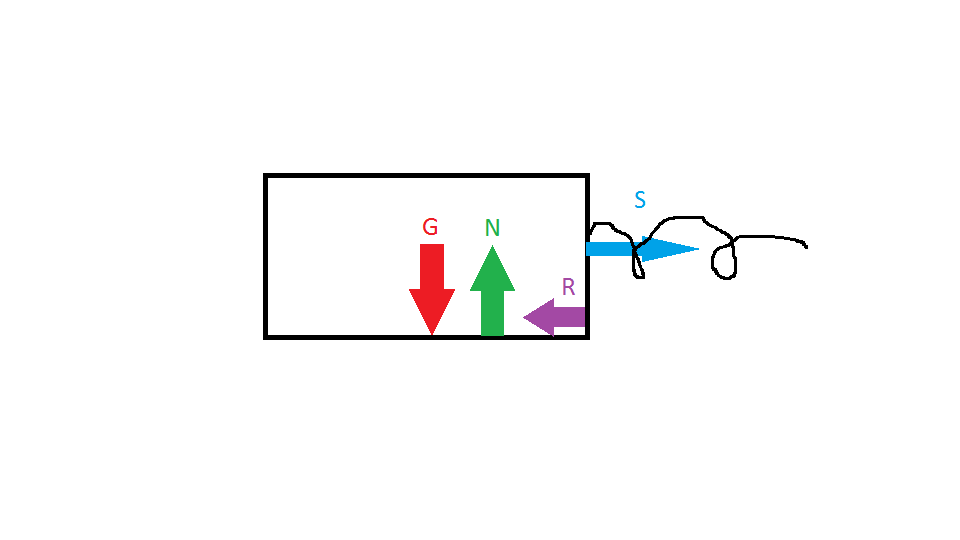
\includegraphics[width=12.6cm,height=8cm]{C:/Users/Torstein/Documents/UiO/Fys-Mek1110/Oblig3_a.png}
			\end{figure}








		\paragraph{b)}
			\begin{flushleft}
Find the position of the spring attachment point $x_b(t)$ as a function of time. \\
\vspace{1mm}
\textbf{Løsning:}
\vspace{1mm}
Punktet $x_b(t)$ er posisjonen $x_0$ som er startposisjonen til høyre side på klossen, pluss hvilelengden til fjera $b$, plussfarten den beveger seg til siden med, ganget med tid.
				\begin{align}
x_b(t) = x_0 + b + ut
				\end{align}
			\end{flushleft}









		\paragraph{c)}
				\begin{flushleft}
Show that the force, $\vec{F}$ on the block from the spring is: $$\vec{F} = k(x_b - x - b)\vec{i}$$. \\
\vspace{1mm}
\textbf{Løsning:} \\
\vspace{1mm}
					\begin{align}
\vec{F} = ks\vec{i} \\
s = x_b - x - b \\
\vec{F} = k(x_b - x - b)\vec{i}
					\end{align}
				\end{flushleft}









		\paragraph{d)}
				\begin{flushleft}
First, let us characterize the stationary state, where the block is moving at a constant velocity. Identify the forces acting on the block and draw a free-body diagram for the block in the stationary state. \\
\vspace{1mm}
\textbf{Løsning:} \\
\vspace{1mm}
				\end{flushleft}
				\begin{figure}[H]
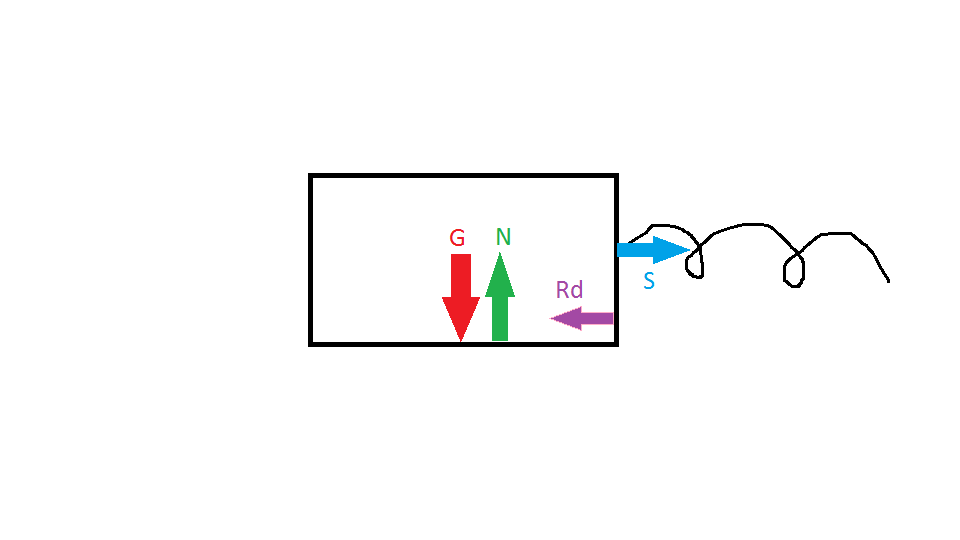
\includegraphics[width=12.6cm,height=8cm]{C:/Users/Torstein/Documents/UiO/Fys-Mek1110/Oblig3_d.png}
				\end{figure}








		\paragraph{e)}
			\begin{flushleft}
Introduce force models for all the forces acting on the block. Find the normal force, $N$, on the block. \\
\vspace{1mm}
\textbf{Løsning:} \\
\vspace{1mm}
				\begin{align}
\vec{S} = k(x_b - x - b)\vec{i} \\
R_d = \mu_d N \\
G = mg \\
N = -mg
				\end{align}
			\end{flushleft}









		\paragraph{f)}
			\begin{flushleft}
Find the acceleration of the block in the stationary state. \\
\vspace{1mm}
\textbf{Løsning:} \\
\vspace{1mm}
I dette tilfellet vil kraften fra fjerden være lik den dynamiske eller statiske friksjonskraften og derfor vil akselrasjonen bli $0$
			\end{flushleft}









		\paragraph{g)}
			\begin{flushleft}
Find the elongation $\Delta L$ of the spring in the stationary state. \\
\vspace{1mm}
\textbf{Løsning:} \\
\vspace{1mm}
				\begin{align}
F = ma = k \Delta L - \mu_d g \\
\Delta L = \frac{\mu_d g m}{k}
				\end{align}
			\end{flushleft}









		\paragraph{h)}
			\begin{flushleft}
Find the position $x(t)$ of the block as a function of time in the stationary state. \\
\vspace{1mm}
\textbf{Løsning:} \\
\vspace{1mm}
Bruker de to likningene for $\Delta L$ og setter inn likningen for $x_b$
				\begin{align}
\frac{\mu_d g m}{k} = x_b(t) - x(t) - b \\
x(t) = -\frac{\mu_d g m}{k} + x_0 + ut
				\end{align}
			\end{flushleft}












		\paragraph{i)}
			\begin{flushleft}
Let us now address the situation where the block starts at rest. That is, we assume that the block starts at $x(t_0) = 0m$ with $v(t_0) = 0m/s$ at the time $t_0 = 0s$. Identify the force acting on the block and draw a free-body diagram of the block before the block starts moving. Introduce force models for all the forces. \\
\vspace{1mm}
\textbf{Løsning:} \\
\vspace{1mm}
				\begin{figure}[H]
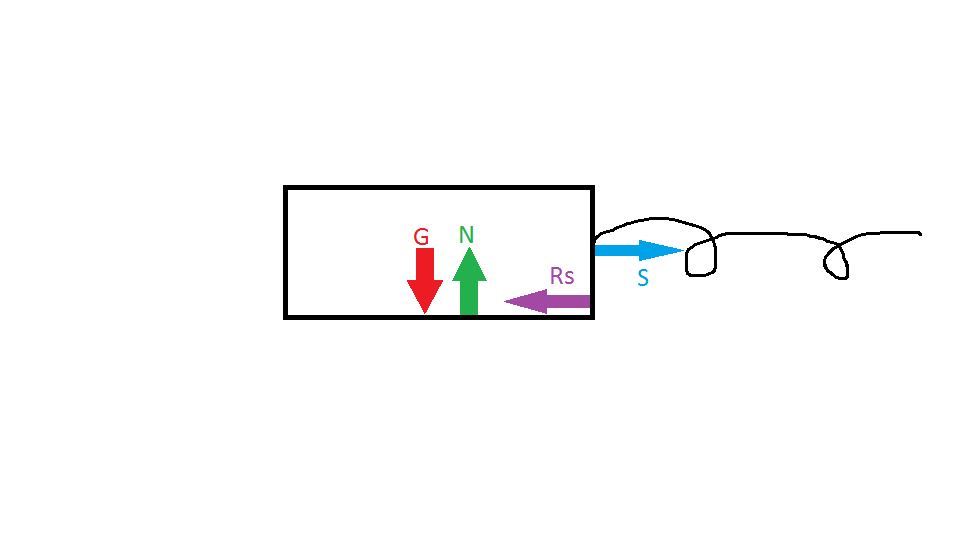
\includegraphics[width=12.6cm,height=8cm]{C:/Users/Torstein/Documents/UiO/Fys-Mek1110/Oblig3_i.png}
				\end{figure}
				\begin{align}
\vec{S} = k(x_b - x - b) \\
R_s \leq -\mu_s mg \\
N = -mg \\
G = mg
				\end{align}
			\end{flushleft}












			\paragraph{j)}
				\begin{flushleft}
Assume that the block starts at rest. Find the elongation $\Delta L$ of the spring at the instant the block starts moving. \\
\vspace{1mm}
\textbf{Løsning:} \\
\vspace{1mm}
				\begin{align}
\vec{S} = R_s \\
k \Delta L = \mu_s mg \\
\Delta L = \frac{\mu_s mg}{k}
				\end{align}
				\end{flushleft}









			\paragraph{k)}
				\begin{flushleft}
Assume that the block starts at rest. Find the friction force on the block as a function in the period before the block starts moving. Sketch the friction force as a function of time until some time after the block has started moving. \\
\vspace{1mm}
\textbf{Løsning:} \\
\vspace{1mm}
					\begin{align}
F_s = S \\
F_s = k(x_b - x - b)
					\end{align}
				\end{flushleft}
				\begin{figure}[H]
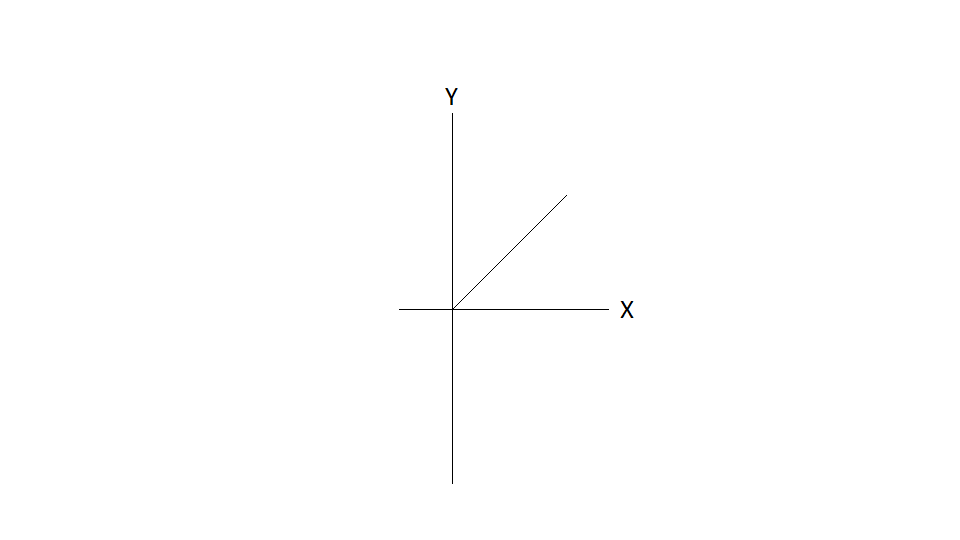
\includegraphics[width=12.6cm,height=8cm]{C:/Users/Torstein/Documents/UiO/Fys-Mek1110/Oblig3_k.png}
				\end{figure}









		\paragraph{l)}
			\begin{flushleft}
Finally, let us address the motion of the block immediately after it starts moving. 
Show that the acceleration of the block immediately after it starts moving is: $$a = \frac{k}{m}(x_b - x - b) - \mu_d g$$ 
Explain why you cannot use this relation for the acceleration to determine the subsequent motion of the block. \\
\vspace{1mm}
\textbf{Løsning:} \\
\vspace{1mm}
				\begin{align}
\sum F = F + F_d \\
ma = k(x_b - x - b)\vec{i} + \mu_d N \\
a = \frac{k(x_0 + b + ut - x - b)}{m} - \mu_d g \\
a = \frac{k(ut - x)}{m} - \mu_d g
				\end{align}
Vi kan ikke bruke denne formelen for akselerasjon fordi vi ikke kjenne
			\end{flushleft}








		\paragraph{m)}
			\begin{flushleft}
Now, we will develop a general method to find the motion of the block. That is, we want to find $x(t)$. We will do this stepwise, checking our results along the way. First, we study the case when $u = 0m/s$ and the coefficients of friction are zero, $\mu_s = \mu_d = 0$. 
Identify the forces acting on the block and draw a free-body diagram of the block. Introduce force models for all the forces. \\
\vspace{1mm}
\textbf{Løsning:} \\
\vspace{1mm}
				\begin{figure}[H]
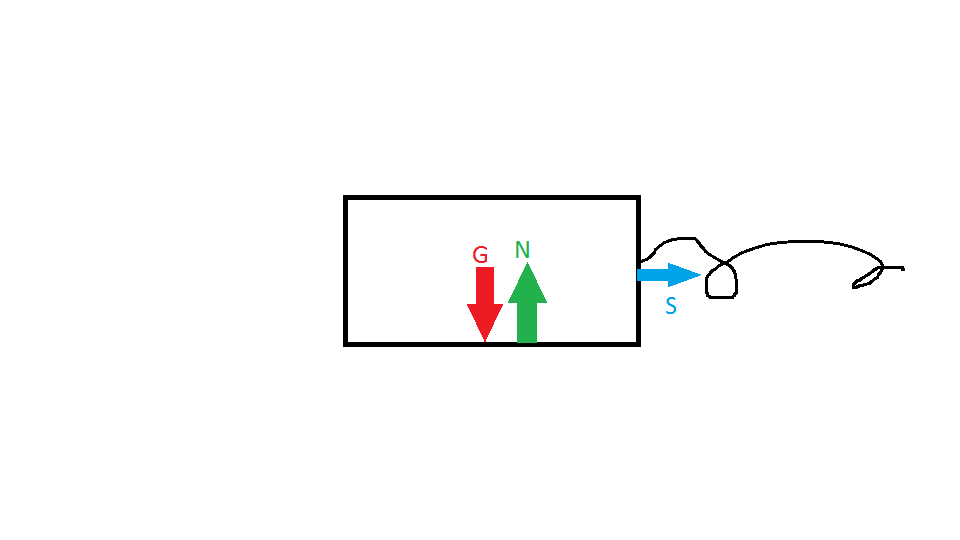
\includegraphics[width=12.6cm,height=8cm]{C:/Users/Torstein/Documents/UiO/Fys-Mek1110/Oblig3_m.png}
				\end{figure}
				\begin{align}
\vec{S} = k(x_b - x - b) \\
N = -mg \\
G = mg
				\end{align}
			\end{flushleft}









		\paragraph{n)}
			\begin{flushleft}
Find an expression for the horizontal acceleration of the block. \\
\vspace{1mm}
\textbf{Løsning:} \\
\vspace{1mm}
				\begin{align}
\sum F = ma \\
ma = k(x_b - x - b) \\
a = \frac{k(x_b - x - b)}{m} = \frac{k}{m}(x_b - x - b) = \frac{k}{m}(x(t))
				\end{align}
			\end{flushleft}






		\paragraph{o)}
			\begin{flushleft}
If the block starts with the velocity $v(t_0) = v(0) = v0$, show that $$x(t) = \frac{v_0}{\omega}sin(\omega t),$$ where $$\omega = \sqrt{\frac{k}{m}},$$ describes the motion of the block – in the case when $u = 0m/s$, and $\mu_s = \mu_d = 0$. \\
\vspace{1mm}
\textbf{Løsning:} \\
\vspace{1mm}
				\begin{align}
a = \frac{k}{m}(-x(t)) \\
x'' - \frac{k}{m}x = 0 \\
r^2 - \frac{k}{m} = 0 \\
r = \frac{\pm \sqrt{-4 \frac{k}{m}}}{2} \Rightarrow r = \pm \sqrt{\frac{k}{m}}\vec{i} \\
x = C cos(\omega t) + D cos(\omega t) \\
0 = C cos(0) + D sin(0) \Rightarrow C = 0 \\
v = D \omega cos(\omega t) \\
v_0 = D \omega \Rightarrow D = \frac{v_0}{\omega} \\
x = \frac{v_0}{\omega}sin(\omega t)
				\end{align}
			\end{flushleft}










		\paragraph{p)}
			\begin{flushleft}
Write a numerical algorithm to find the position and velocity of the block at a time $t_i + \Delta t, x(t_i + \Delta t)$ and $v(t_i + \Delta t)$, given the position and velocity of the block at a time $t_i, x(t_i)$ and $v(t_i)$. \\
\vspace{1mm}
\textbf{Løsning:} \\
\vspace{1mm}
\lstinputlisting{oblig3_p.py}
			\end{flushleft}










		\paragraph{q)}
			\begin{flushleft}
Implement the numerical algorithm in a program to find the position of the block as a function of time for $m = 0.1kg$, $k = 100N/m$, $b = 0.1m$ and $v0 = 0.1m/s$. Plot the behavior for a simulation of $2s$, and compare the result of your program with with exact solution. Ensure that you choose a time-step $\Delta t$ the reproduces the exact solution with sufficient accuracy. What happens if you choose a too large time-step $\Delta t$? \\
\vspace{1mm}
\textbf{Løsning:} \\
\vspace{1mm}
\lstinputlisting{oblig3_q.py}
				\begin{figure}[H]
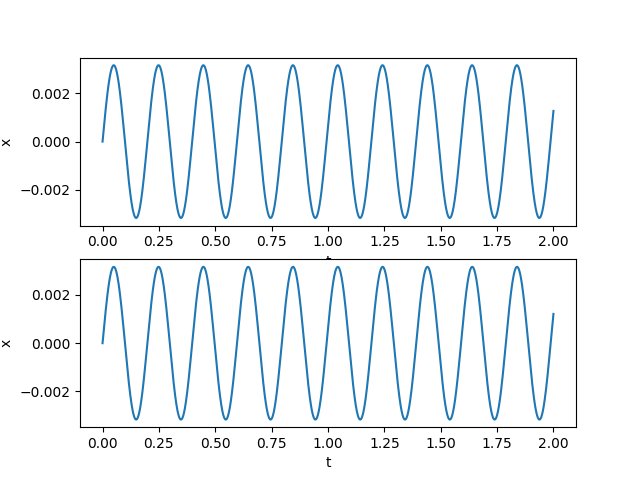
\includegraphics[width=12.6cm,height=8cm]{oblig3_q.png}
				\end{figure}
Hvis du velger et for stort tidssteg vil programmet ta veldig lang tid å kjøre.
			\end{flushleft}













		\paragraph{r)}
			\begin{flushleft}
Modify your program to find the position of the block when $u = 0.1m/s$ and the block starts at rest. In this case, the exact solution is: $$x(t) = ut - \frac{u}{\omega} sin \omega t.$$ Compare your result with the exact solution by plotting both the simulated $x$ and the exact $x$ in the same plot. \\
\vspace{1mm}
\textbf{Løsning:} \\
\vspace{1mm}
\lstinputlisting{oblig3_r.py}
				\begin{figure}[H]
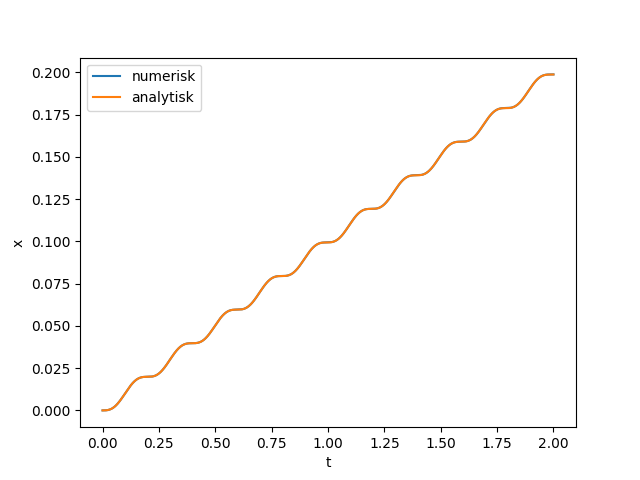
\includegraphics[width=12.6cm,height=8cm]{oblig3_r.png}
				\end{figure}
Vi ser av bildet over at den numeriske analysen og den analytiske analysen ga helt like svar.
			\end{flushleft}







		\paragraph{s)}
			\begin{flushleft}
Finally, we address the full complexity of the situation, and introduce non-zero friction forces.
Modify your program to include friction using $\mu_s = 0.6$, $\mu_d = 0.3$. Show a plot of $x(t)$ for $m = 0.1kg$ and for $m = 1.0kg$. \\
\vspace{1mm}
\textbf{Løsning:} \\
\vspace{1mm}
\lstinputlisting{oblig3_s.py}
				\begin{figure}[H]
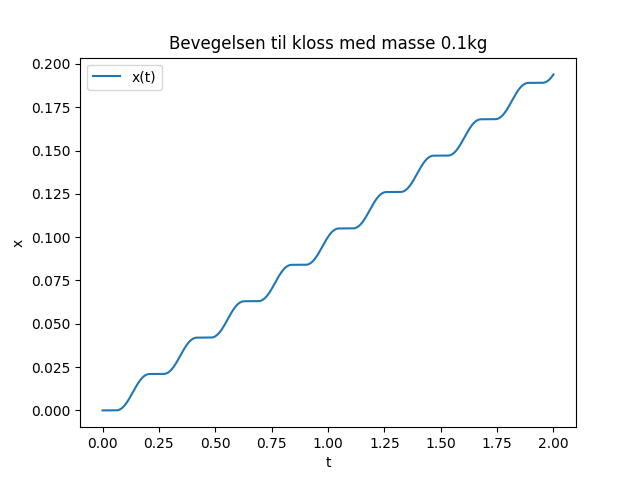
\includegraphics[width=12.6cm,height=8cm]{oblig3_s1.png}
				\end{figure}
				\begin{figure}[H]
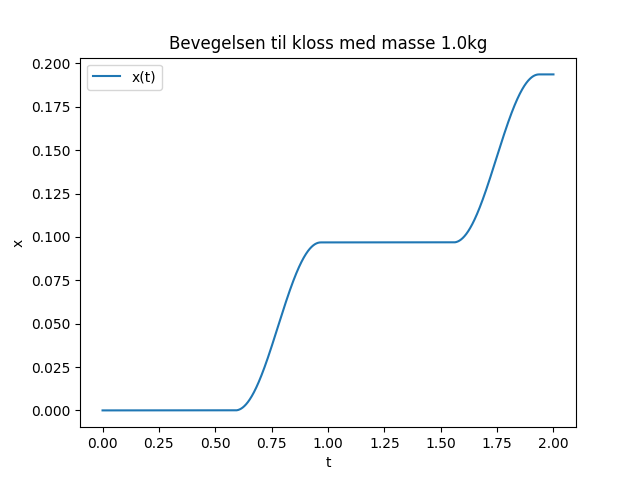
\includegraphics[width=12.6cm,height=8cm]{oblig3_s2.png}
				\end{figure}
			\end{flushleft}










		\paragraph{t)}
		\begin{flushleft}
You should also plot the spring force F on the block as a function of time for both cases in the previous exercise. Can you explain the differences? \\
\vspace{1mm}
\textbf{Løsning:} \\
\vspace{1mm}
\lstinputlisting{oblig3_t.py}
			\begin{figure}[H]
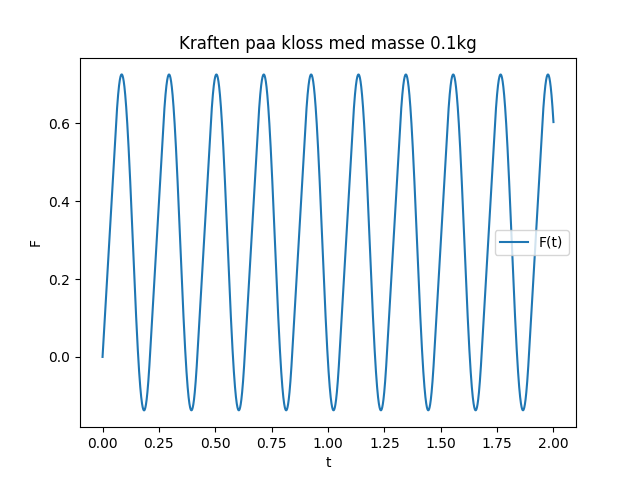
\includegraphics[width=12.6cm,height=8cm]{oblig3_t1.png}
			\end{figure}
			\begin{figure}[H]
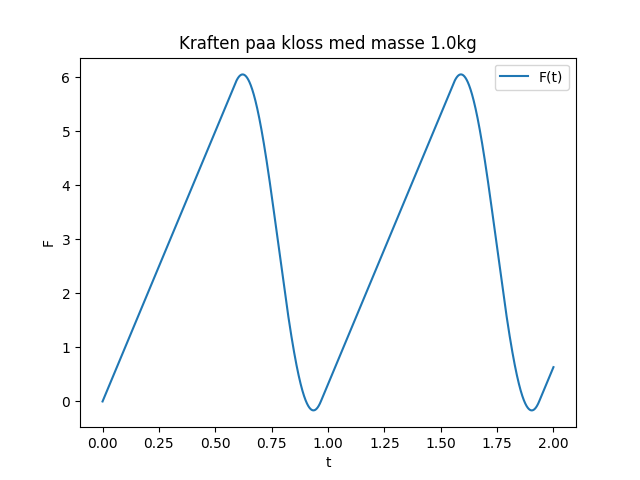
\includegraphics[width=12.6cm,height=8cm]{oblig3_t2.png}
			\end{figure}
Forskjellen kommer av at vekten gjør at det tar mye lenger tid å flytte den tunge klossen enn den lette over det samme strekket med den samme kraften.
		\end{flushleft}










		\paragraph{u)}
		\begin{flushleft}
What happens if you instead decrease $k$ to $k = 10N$ for $m = 0.1kg$. Can you explain the behavior?\\
\vspace{1mm}
\textbf{Løsning:} \\
\vspace{1mm}
\lstinputlisting{oblig3_u.py}
			\begin{figure}[H]
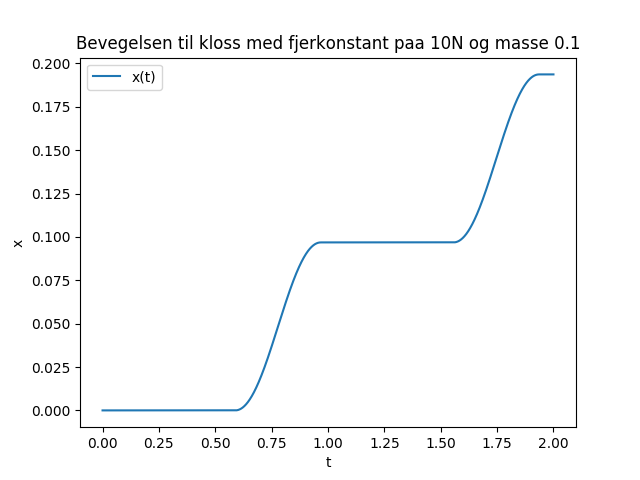
\includegraphics[width=12.6cm,height=8cm]{oblig3_u.png}
			\end{figure}
Bevegelsen blir den samme som for $k = 100N$ og $m = 1.0kg$ dette kommer av at det eneste disse to tingene har en effekt på er akselrasjonen og i formelen for akselrasjon ser de slik ut: $\frac{k}{m}$. Her ser vi at hundre delt på en er det samme som ti delt på $0.1$.
		\end{flushleft}
\end{document}